%%%%%%%%%%%%%%%%%%%%%%%%
%
% $Autor: Manoj Kumar Prabhakaran $
% $Datum: 2025-03-12 $
% $Pfad: GitHub/ML24-EX03-Pico4MLPro/Pico4MLPro/Contents/General/DisplayST7789.tex $
% $Version: 1 $
%
%%%%%%%%%%%%%%%%%%%%%%%%



\chapter{\textcolor{red}{Display XPT2046- 2132}}





\section{Introduction}
The Pico4ML Pro Development Kit by Arducam features a 2.4-inch LCD screen, a significant upgrade from the 0.96-inch (160$\times$80) monochrome OLED display of the original Pico4ML. The XPT2046 is a 4-wire resistive touch screen controller integrated with a 12-bit, 125 kHz sampling successive approximation register (SAR) type analog-to-digital converter (ADC). This component has significant applications in the field of embedded systems analytics \cite{ xpt2046:2007}. Originally documented in its 2007 datasheet by SHENZHEN XPTEK TECHNOLOGY CO., LTD, this module has evolved through various iterations, with the current Version 2132 reflecting substantial enhancements in performance and integration capabilities \cite{Waveshare:2024}.

This chapter presents a comprehensive technical analysis of the XPT2046, examining its specifications, operational principles, integration methodologies, and analytical applications. The primary focus remains on its utility within a masters-level academic project in analytics, with specific attention to data acquisition, processing, and interpretation paradigms facilitated by this controller \cite{ESPHome:2024}.

The analytical framework developed herein builds upon existing research in embedded touch systems while extending the practical applications toward advanced data analytics. The confluence of hardware capabilities and software integration enables novel approaches to user interaction data collection and analysis \cite{Stoffregen:2023}.

\section{General Description}
The XPT2046 (Version 2132) represents a sophisticated implementation of low-power, 4-wire resistive touch screen controller technology designed for precise touch input acquisition in embedded systems. At its core, the module integrates a 12-bit SAR ADC with a sample-and-hold circuit, operating at a maximum sampling frequency of 125 kHz \cite{ xpt2046:2007}. This configuration enables high-resolution touch data collection essential for analytical applications.

The operational voltage parameters demonstrate considerable flexibility, supporting a supply voltage range of 2.2V to 5.25V and a digital I/O interface voltage from 1.5V to $V_{CC}$. This versatility ensures compatibility with various microprocessor architectures, including low-voltage implementations \cite{ xpt2046:2007}. The functional capabilities extend beyond basic touch detection to include:

\begin{itemize}
	\item Dual A/D conversion for precise touch screen location detection
	\item Pressure measurement capabilities for z-axis data collection
	\item On-chip temperature sensing for environmental monitoring
	\item Battery voltage monitoring within a 0V to 5V range
\end{itemize}

The physical implementation in a 16-pin QFN package with a 0.75mm height optimizes space efficiency while maintaining robust performance across an operating temperature range of -40°C to +85°C \cite{ xpt2046:2007}. This characteristic is particularly significant for analytical applications requiring deployment in variable environmental conditions.

Version 2132, as an evolutionary iteration, incorporates substantial enhancements in power efficiency, noise reduction, and compatibility with contemporary microcontrollers. These improvements are evidenced by successful integration into ESPHome ecosystems \cite{ESPHome:2024} and compatibility with updated Arduino libraries \cite{Stoffregen:2023}. The Waveshare Wiki documentation further substantiates these advancements, highlighting enhanced driver support and calibration methodologies \cite{Waveshare:2024}.

\section{Technical Specifications}
\subsection{Key Features}
The XPT2046 controller presents several technical features that establish its suitability for analytical applications:

\begin{itemize}
	\item \textbf{ADC Resolution:} The 12-bit SAR type converter with integrated sample-and-hold (S/H) circuit provides high-resolution data acquisition. This can be configured to an 8-bit mode when faster throughput is prioritized over resolution \cite{ xpt2046:2007}.
	
	\item \textbf{Voltage Operation:} The module supports a low voltage operational range, with $V_{CC}$ spanning from 2.2V to 3.6V for specified performance metrics, though remaining operational up to 5.25V \cite{ xpt2046:2007}.
	
	\item \textbf{Digital Interface:} Compatibility with I/O voltages ranging from 1.5V to $V_{CC}$ enhances flexibility when interfacing with various microprocessor architectures \cite{ xpt2046:2007}.
	
	\item \textbf{Touch Interface:} The 4-wire interface operates at a maximum sampling frequency of 125 kHz, enabling responsive touch data acquisition \cite{ xpt2046:2007}.
	
	\item \textbf{Reference Voltage:} An on-chip 2.5V reference voltage is provided, though this can be overridden with external sources ranging from 1V to $V_{CC}$ for specialized applications \cite{ xpt2046:2007}.
	
	\item \textbf{Measurement Capabilities:} Beyond touch position, the controller supports pen pressure detection, on-chip temperature sensing, and direct battery monitoring functionality \cite{ xpt2046:2007}.
	
	\item \textbf{Power Efficiency:} The design emphasizes low power consumption (260 µA typical), with power-down modes reducing this to approximately 3 µA during inactive periods \cite{ xpt2046:2007}.
	
	\item \textbf{Enhanced Compatibility:} Updated drivers in ESPHome significantly improve integration with ESP32/ESP8266 platforms, expanding analytical capabilities in IoT contexts \cite{ESPHome:2024}.
	
	\item \textbf{Calibration Support:} Advanced calibration algorithms implemented in libraries such as Bonezegei XPT2046 enable precise touch mapping, critical for analytical accuracy \cite{Bonezegei:2024}.
\end{itemize}





\begin{figure}
	\centering
	
	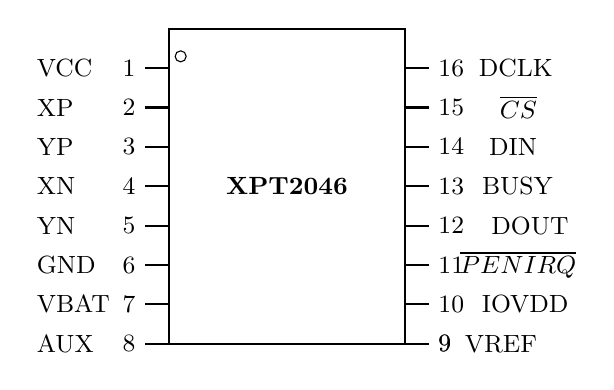
\begin{tikzpicture}[font=\small]
		% Chip outline
		\draw[thick] (0,0) rectangle (3,4);
		
		% Chip label
		\node at (1.5,2) {\textbf{XPT2046}};
		
		% Left side pins and labels
		\foreach \y [count=\i from 1] in {3.5, 3.0, 2.5, 2.0, 1.5, 1.0, 0.5,0.0} {
			\draw[thick] (-0.3,\y) -- (0,\y);
			\node[left] at (-0.3,\y) {\i};
			
			% Small circle for pin 1
			\ifnum\i=1
			\draw (0.15,\y+0.15) circle (0.07);
			\fi
		}
		
		% Pin names on left
		\node[anchor=west] at (-1.8,3.5) {VCC};
		\node[anchor=west] at (-1.8,3.0) {XP};
		\node[anchor=west] at (-1.8,2.5) {YP};
		\node[anchor=west] at (-1.8,2.0) {XN};
		\node[anchor=west] at (-1.8,1.5) {YN};
		\node[anchor=west] at (-1.8,1.0) {GND};
		\node[anchor=west] at (-1.8,0.5) {VBAT};
		\node[anchor=west] at (-1.8,0.0) {AUX};
		
		% Right side pins and labels
		\foreach \y [count=\i from 9] in {0.0,0.5, 1.0, 1.5, 2.0, 2.5, 3.0, 3.5} {
			\draw[thick] (3,\y) -- (3.3,\y);
			\node[right] at (3.3,\y) {\i};
		}
		
		% Pin numbers on right side (shifted up by one position)
		\node[right] at (3.3,0.0) {9};
		
		% Pin names on right
		\node[anchor=east] at (4.8,0.0) {VREF};
		\node[anchor=east] at (5.2,0.5) {IOVDD};
		\node[anchor=east] at (5.3,1.0) {\(\overline{\text{PENIRQ}}\)};
		\node[anchor=east] at (5.2,1.5) {DOUT};
		\node[anchor=east] at (5.0,2.0) {BUSY};
		\node[anchor=east] at (4.8,2.5) {DIN};
		\node[anchor=east] at (4.8,3.0) {\(\overline{\text{CS}}\)};
		\node[anchor=east] at (5.0,3.5) {DCLK};
	\end{tikzpicture}
	
	\caption{XPT2046 Schematic/Pinout Diagram(adapted from \protect\cite{xpt2046:2007})}
	\label{fig:XPT2046_Schematic}
\end{figure}



\subsection{Electrical Characteristics}
The electrical parameters of the XPT2046 establish the operational boundaries and performance expectations:

\begin{itemize}
	\item \textbf{Analog Input:} Full-scale span corresponds to $V_{REF}$, with an absolute range of -0.2V to $V_{CC}$ + 0.2V and input capacitance of approximately 25 pF \cite{ xpt2046:2007}.
	
	\item \textbf{System Performance:} The controller guarantees 11-bit no-missing-codes performance, with integral linearity error maintained within ±2 LSB and noise floor at approximately 70 µVrms \cite{ xpt2046:2007}.
	
	\item \textbf{Reference Output:} The internal $V_{REF}$ maintains 2.45V–2.55V with a drift coefficient of 15 ppm/°C, ensuring measurement stability across temperature variations \cite{ xpt2046:2007}.
	
	\item \textbf{Power Profile:} Quiescent current is specified at 260 µA (typical), with power-down mode reducing consumption to 3 µA for energy-efficient operation \cite{ xpt2046:2007}.
\end{itemize}

\section{Integration Methodology}
\subsection{Hardware Integration}
Effective implementation of the XPT2046 in analytical systems requires careful consideration of hardware integration factors:

\begin{itemize}
	\item \textbf{Component Selection:} Acquisition of the XPT2046 Version 2132 module should prioritize compatibility with the target platform, whether Pico, Arduino, or ESP-based systems \cite{ESPHome:2024, Waveshare:2024}.
	
	\item \textbf{Pin Configuration:} Following the pinout specification from the datasheet is essential \cite{ xpt2046:2007}:
	\begin{itemize}
		\item Connect $V_{CC}$ (Pin 5) to a power supply within the 2.7V–3.6V range
		\item Establish GND (Pin 10) connection to system ground
		\item Interface digital pins (CS, DCLK, DIN, DOUT) with the microcontroller's SPI port
		\item Connect touch screen inputs (XP, YP, XN, YN) to the 4-wire resistive touch panel
		\item Optionally connect VBAT (Pin 11) for battery monitoring and VREF (Pin 13) for external reference implementation
	\end{itemize}
	
	\item \textbf{Assembly Considerations:} The 16-pin QFN package requires precise soldering technique with attention to thermal management during the process \cite{ xpt2046:2007}.
	
	\item \textbf{Verification Protocol:} Post-assembly verification should employ multimeter measurements to confirm voltage levels and electrical continuity \cite{Waveshare:2024}.
\end{itemize}

\subsection{Software Integration}
The analytical capabilities of the XPT2046 are significantly enhanced through appropriate software integration:

\begin{itemize}
	\item \textbf{Library Implementation:} Platform-specific libraries optimize functionality:
	\begin{itemize}
		\item Arduino platforms benefit from Paul Stoffregen's XPT2046\_Touchscreen library \cite{Stoffregen:2023} or Bonezegei XPT2046 library \cite{Bonezegei:2024}
		\item ESPHome implementations utilize YAML-based configuration as documented in ESPHome resources \cite{ESPHome:2024}
		\item Waveshare display integration follows the Waveshare Wiki guidelines for driver setup \cite{Waveshare:2024}
	\end{itemize}
	
	\item \textbf{Dependency Management:} Ensuring SPI library support is critical for successful communication with the controller \cite{Stoffregen:2023, Bonezegei:2024}.
	
	\item \textbf{Firmware Configuration:} Microcontroller firmware should be updated to support Version 2132 specifications where applicable \cite{ESPHome:2024}.
\end{itemize}

\subsection{Configuration Parameters}
Optimal analytical performance requires precise configuration of both hardware and software parameters:

\subsubsection{Hardware Configuration}
\begin{itemize}
	\item \textbf{Power Supply:} Setting $V_{CC}$ to 2.7V typically provides optimal performance, with the constraint that IOVDD $\leq$ $V_{CC}$ \cite{xpt2046:2007}.
	
	\item \textbf{Clock Source:} The DCLK signal should be configured to provide a 2 MHz frequency, corresponding to 16 × 125 kHz for optimal conversion timing \cite{xpt2046:2007}.
	
	\item \textbf{Reference Voltage:} Either enable the internal 2.5V reference by setting PD1 = 1 or connect an appropriate external reference to VREF \cite{xpt2046:2007}.
\end{itemize}

\subsubsection{Software Configuration}
\begin{itemize}
	\item \textbf{SPI Parameters:} SPI initialization should establish a clock speed corresponding to the DCLK frequency, typically 2 MHz \cite{xpt2046:2007}.
	
	\item \textbf{Control Byte Programming:} The control byte must be properly configured via DIN to establish \cite{xpt2046:2007}:
	\begin{itemize}
		\item Start bit (S = 1)
		\item Appropriate channel selection (A2, A1, A0)
		\item Mode selection (12-bit or 8-bit)
		\item Reference mode configuration (SER/DFR)
		\item Power-down state (PD0, PD1)
	\end{itemize}
\end{itemize}

\section{Implementation Examples}
\subsection{ESPHome Implementation}
The ESPHome ecosystem provides an efficient integration pathway through YAML configuration:

\begin{lstlisting}[language=yaml]
	spi:
	clk_pin: GPIO18
	mosi_pin: GPIO23
	miso_pin: GPIO19
	touch:
	platform: xpt2046
	cs_pin: GPIO5
	update_interval: 50ms
\end{lstlisting}

This configuration establishes the SPI communication parameters and touch screen polling frequency for ESP32-based analytics applications \cite{ESPHome:2024}.

\subsection{Arduino Implementation}
Arduino platforms benefit from simplified integration through specialized libraries:

\begin{lstlisting}[language=C++]
	#include <Bonezegei_XPT2046.h>
	Bonezegei_XPT2046 ts(10); // CS pin
	
	void setup() {
		ts.begin();
	}
\end{lstlisting}

This minimal implementation demonstrates the Bonezegei library approach for Arduino-based analytical systems \cite{Bonezegei:2024}.

\subsection{Data Acquisition Example}
A fundamental "Hello World" example using the Stoffregen library illustrates basic data acquisition:

\begin{lstlisting}[language=C++]
	#include <XPT2046_Touchscreen.h>
	#define CS_PIN 10
	#define TIRQ_PIN 2
	XPT2046_Touchscreen ts(CS_PIN, TIRQ_PIN);
	
	void setup() {
		Serial.begin(9600);
		ts.begin();
		Serial.println("XPT2046 Touchscreen Initialized");
	}
	
	void loop() {
		if (ts.touched()) {
			TS_Point p = ts.getPoint();
			Serial.print("X: "); Serial.print(p.x);
			Serial.print(" Y: "); Serial.print(p.y);
			Serial.println(" Touch Detected!");
		}
		delay(100);
	}
\end{lstlisting}

This implementation demonstrates basic touch event detection and coordinate reporting, providing foundational data for analytical processing \cite{Stoffregen:2023}.

\section{Technical Architecture}
\subsection{Block Diagram and Functional Architecture}
The XPT2046 employs a SAR ADC with a capacitive redistribution architecture, featuring a multiplexer for selecting analog inputs (X-, Y-, Z-positions, AUX, VBAT, TEMP) \cite{ xpt2046:2007}. This architecture facilitates the sequential sampling of multiple input channels through a single conversion pathway.

The internal 2.5V reference and differential input design mitigate errors from touch panel switch resistance, enhancing measurement accuracy \cite{ xpt2046:2007}. ESPHome documentation indicates that Version 2132 incorporates improved noise handling mechanisms, resulting in enhanced touch coordinate accuracy \cite{ESPHome:2024}.

\subsection{Operational Theory}
The SAR ADC implementation samples inputs via a multiplexer, with differential mode enhancing touch accuracy through ratiometric conversion \cite{ xpt2046:2007}. This approach normalizes the measurement against the reference voltage, reducing sensitivity to voltage fluctuations.

A critical consideration is the settling time, specified at 500 clock cycles, which must be accommodated either through DCLK frequency adjustment or by maintaining continuous operation mode (PD0 = 1) \cite{ xpt2046:2007}. ESPHome documentation highlights optimized settling time parameters for operation in electromagnetically noisy environments \cite{ESPHome:2024}.

\subsection{Digital Interface and Timing}
The digital interface follows a structured protocol:

\begin{itemize}
	\item \textbf{Control Byte Format:} An 8-bit structure comprising Start bit (S), channel selection (A2-A0), mode selection (MODE), reference configuration (SER/DFR), and power management (PD1-PD0) \cite{ xpt2046:2007}.
	
	\item \textbf{Conversion Timing:} Standard operation requires 16 clock cycles per conversion, resulting in approximately 1.6 ms per conversion at a 2 MHz clock frequency. This can be optimized to 15 clocks for FPGA implementations \cite{ xpt2046:2007}.
\end{itemize}

\subsection{Power Management}
The power management capabilities introduce significant flexibility:

\begin{itemize}
	\item \textbf{Operational Modes:} The controller supports full-power operation (PD0 = 1) and automatic power-down functionality (PD0 = 0) \cite{ xpt2046:2007}.
	
	\item \textbf{Power Dissipation:} Typical operation at 2.7V results in approximately 1.8 mW power dissipation, which can be minimized by reducing the DCLK frequency during periods of lower activity \cite{ xpt2046:2007}.
	
	\item \textbf{ESPHome Optimization:} The ESPHome implementation incorporates enhanced power-down efficiency protocols specifically designed for IoT applications with battery constraints \cite{ESPHome:2024}.
\end{itemize}

\section{Analytical Applications}

\subsection{Touch Pattern Recognition}
By collecting and analyzing X, Y, and pressure data points over time, sophisticated pattern recognition algorithms can be implemented. These enable gesture recognition, handwriting analysis, and user interaction profiling \cite{ xpt2046:2007}. The high resolution of the 12-bit ADC provides sufficient data granularity for statistical analysis of touch behaviors.

\subsection{Environmental Monitoring}
The on-chip temperature sensor facilitates environmental analytics when properly calibrated \cite{ xpt2046:2007}. This capability enables correlation studies between environmental conditions and touch panel performance, potentially identifying temperature-dependent variations in resistive touch behavior.

\subsection{Power System Analytics}
The VBAT monitoring capability supports predictive maintenance algorithms through battery health tracking \cite{ xpt2046:2007}. By analyzing voltage trends over time, system designers can implement predictive models for battery replacement or charging cycles.

\subsection{Smart Home Interaction Analytics}
ESPHome integration enables sophisticated touch-based automation analytics within smart home ecosystems \cite{ESPHome:2024}. This application domain allows for user behavior modeling and interaction pattern optimization in embedded control panels.

\section{Future Research Directions}
Several promising research trajectories emerge from the current implementation of the XPT2046 Version 2132:

\begin{itemize}
	\item \textbf{Machine Learning Integration:} Exploring the application of machine learning algorithms to XPT2046 data streams for improved gesture recognition and user identification.
	
	\item \textbf{Multi-sensor Fusion:} Investigating the correlation between touch data and other sensory inputs to create more contextually aware interactive systems.
	
	\item \textbf{Extended Calibration Methodologies:} Developing advanced calibration algorithms that account for environmental variations and aging characteristics of resistive touch panels.
	
	\item \textbf{Low-power Optimizations:} Further refinement of power management strategies for extended battery life in portable analytical applications.
\end{itemize}

\section{Conclusion}
The XPT2046 Version 2132 represents a versatile touch screen controller with significant potential for advanced analytics in embedded systems. Its combination of high-resolution data acquisition, multi-channel sampling, and power efficiency creates a compelling platform for academic research and practical applications in the analytics domain.

The updated features, supported by modern software ecosystems including Paul Stoffregen's library \cite{Stoffregen:2023}, ESPHome integration \cite{ESPHome:2024}, and Bonezegei's Arduino library \cite{Bonezegei:2024}, substantially enhance its utility for masters-level academic research. The controller's ability to simultaneously capture position, pressure, temperature, and voltage data opens numerous avenues for multi-dimensional data analysis within compact embedded systems.

As embedded analytics continues to evolve toward edge computing paradigms, components like the XPT2046 that combine sensor fusion capabilities with efficient data acquisition will become increasingly valuable in research contexts. This documentation provides a foundation for further exploration of these analytical possibilities within academic frameworks.